\documentclass[]{article}
\usepackage[utf8]{inputenc}
\usepackage{setspace}
\usepackage{epsfig}    
\usepackage{amsfonts}
\usepackage{amssymb}
\usepackage{amsmath}
\usepackage{subfigure}
\usepackage{comment}
\usepackage{multirow}
\usepackage{soul} 
\usepackage[dvipsnames]{xcolor}
\usepackage{hyperref}
\usepackage{color}
\usepackage{mathtools}
\usepackage{fullpage}
\usepackage{algorithmic}
\DeclareMathOperator*{\argmin}{argmin}
\algsetup{linenosize=\small}
\usepackage{cite}
\usepackage{setspace}
\usepackage{textcomp}
\usepackage{xspace}
\usepackage{siunitx}
\usepackage{epstopdf}
\usepackage{url}
\usepackage{dblfloatfix}
\usepackage[toc,page]{appendix}

\DeclareMathOperator{\E}{\mathbb{E}} % Expectation Symbol
\usepackage[linesnumbered,ruled]{algorithm2e}
\usepackage{booktabs}
\usepackage{hyperref}

\usepackage{tcolorbox}

\newtcolorbox{mybox}[3][]
{
	colframe = #2!25,
	colback  = #2!10,
	coltitle = #2!20!black,  
	title    = #3,
	#1,
}

\begin{document}
	
	\title{Implementation of the IEEE 802.11ax Spatial Reuse Operation in Komondor}
	\author{Author}
	
	%\institute{Department of Information and Communication Technologies, \\Universitat Pompeu Fabra, Barcelona\\
	%\email{\{author\}@upf.edu}
	%}
	\date{}
	
	\maketitle
	
	% SUBFIGURE EXAMPLE
	%	\begin{figure*}
	%		\centering
	%		\subfigure[Scenario]{\label{fig:11ax_bss_coloring_a}\includegraphics[width=50mm]{img/11ax_bss_coloring_a}}
	%		\subfigure[Packets exchange]{\label{fig:11ax_bss_coloring_b}\includegraphics[width=110mm]{img/11ax_bss_coloring_b}}
	%		\caption{Channel access rules based on the BSS Color inspected in the incoming packets.}
	%	\end{figure*}	
	
	% FIGURE EXAMPLE
	%	\begin{figure*}[h!]
	%		\centering
	%		\epsfig{file=img/two_navs.pdf, width=10cm}
	%		\caption{Intra and inter-BSS frames exchange. Both $\text{AP}_0$ and $\text{AP}1$ send an HE PPDU indicating their BSS\_COLOR, which allows to $\text{STA}_{0.1}$ to determine which are intra and inter-BSS frames, thus setting different NAV values. On the other hand, $\text{AP}_2$ does not support BSS coloring, but indicates its BSSID, which is useful to the same purpose.}
	%		\label{fig:two_navs}
	%	\end{figure*}	
	
	\begin{abstract}
		This document is aimed at providing an explanation on the implementation carried about in Komondor to simulate the Spatial Reuse (SR) operation included in the IEEE 802.11ax amendment. In addition to detail the main implemented functionalities, several validations are provided. All the source code can be found at \url{www.github.com/wn-upf/Komondor}
	\end{abstract}
	
	% ----------------------------------
	% -
	% 	-- Intra and Inter-BSS frames --
	% -
	% ----------------------------------
	
	\section{Intra and Inter-BSS frames} 
	\label{section:intra_inter_bss_frames}
	
	\subsection{Implementation}
	
	In order to implement the 11ax SR operation, we first need to be able to differentiate between intra and inter-BSS frames. To that purpose, we have added extra conditions at the following points, where the detected transmission is inspected:
	\begin{itemize}
		\item When a node is in state ``Sensing" and a new transmission is detected: 
		\begin{itemize}
			\item The packet is of type RTS or CTS, and despite the current node is not the packet destination, it can be decoded.
			\item The packet is of type DATA or ACK. 
		\end{itemize}
		\item When a node is in state ``NAV":
		\begin{itemize}
			\item The packet is of type RTS or CTS, and despite the current node is not the packet destination, it can be decoded. In addition, no collisions by backoff are noticed.
		\end{itemize}
	\end{itemize}
	
	If any of the abovementioned situations occur, the node of interest checks the BSS color and the Spatial Reuse Group (SRG) fields. The frame is categorized as an \textbf{intra-BSS PPDU} if \emph{i)} the BSS color of the received packet matches with the BSS color of the node, or \emph{ii)} the SRG matches with the SRG to which the node belongs. 
	
	Both BSS color and SRG fields are indicated in the ``input\_nodes" file. Those fields are not mandatory. In case of not including them, Komondor considers that the attributes BSS Color and SRG of a given node are 0. When either BSS Color and/or SRG fields are 0, the SR operation is disabled.
	
	\begin{mybox}{red}{ALERT}
		%\centering
		\textbf{The following important assumption has been done:} Packet inspection is assumed to be done at the beginning, which is not actually true. In fact, an HE STA that detects a PPDU spends some time inspecting the BSS Color field, which is in the HE-SIG-A PHY header.		
	\end{mybox}
	
	\begin{mybox}{red}{ALERT}
		%\centering
		\textbf{The following important assumption has been done:} The SRG is virtually indicated in every packet. However, in reality the SRG is maintained in the BSS Color Bitmap, which is checked according to the received BSS Color.		
	\end{mybox}
	
	\subsection{Validation}
	
	In order to validate the proper intra and inter-BSS frames operation, we propose the following two scenarios:	
	\begin{itemize}
		\item Scenario 1: One WLAN, containing 1 AP and 2 STAs (Figure \ref{fig:scenario_1_1}).
		\item Scenario 2: Two WLANs, containing 1 AP and 1 STA each (Figure \ref{fig:scenario_1_2}).
	\end{itemize}
	
	\begin{figure*}
		\centering
		\subfigure[Scenario 1]{\label{fig:scenario_1_1}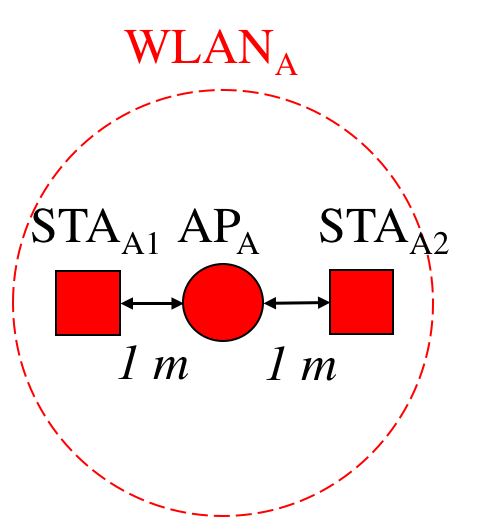
\includegraphics[width=35mm]{img/scenario_1_1}}
		\subfigure[Scenario 2]{\label{fig:scenario_1_2}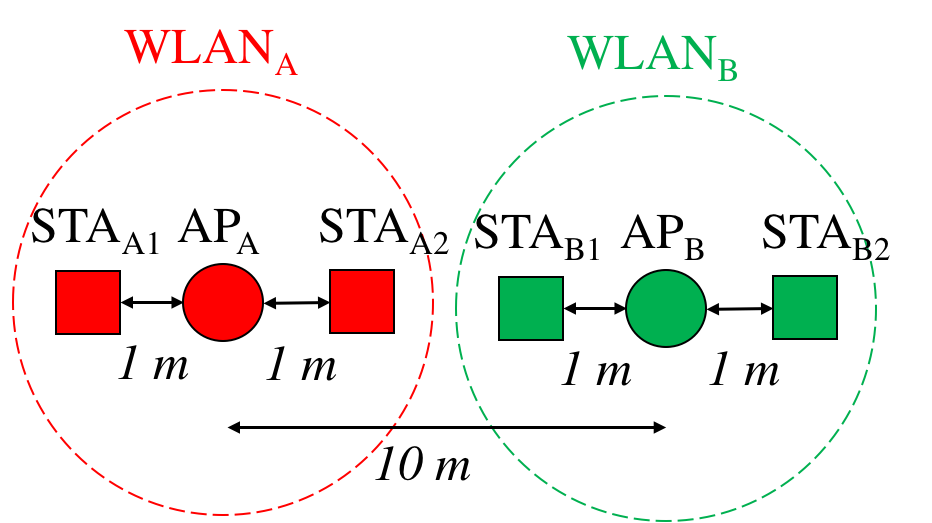
\includegraphics[width=65mm]{img/scenario_1_2}}
		\subfigure[Scenario 3]{\label{fig:scenario_1_3}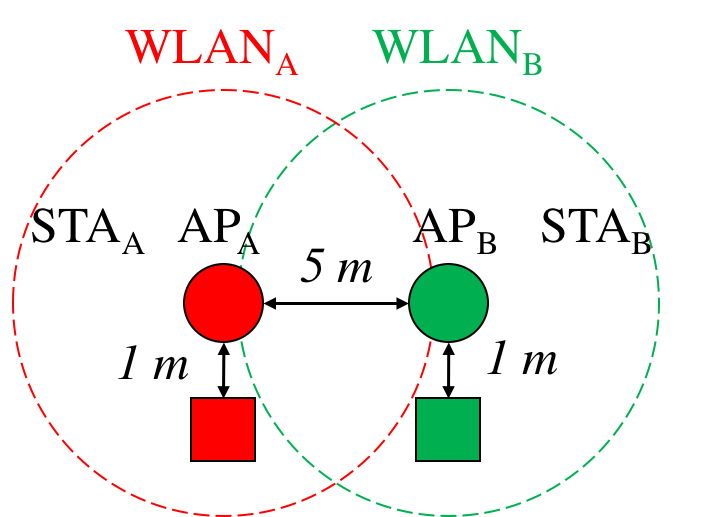
\includegraphics[width=50mm]{img/scenario_1_3}}
		\caption{Scenarios for validating intra and inter-BSS frames}
	\end{figure*}	
	
	What we want to do in Scenarios 1 and 2, is to check that no inter-BSS frames are detected, since transmitters are not in range of any other WLAN using a different BSS color or SRG. In contrast, in Scenario 3 we aim to check that PPDUs are properly classified in each node. To that purpose, we allow nodes to ignore inter-BSS PPDUs if the received power is lower than a given OBSS\_PD threshold. In 3a, OBSS\_PD is set to -62 dBm, thus allowing to ignore all the inter-BSS PPDUs, while in 3b, OBSS\_PD is set to -82 dBm, which is not enough to ignore the OBSS transmissions. The summarized results for each scenario are shown in Table \ref{tbl:results_part_1}.
	
	\begin{table}[]
		\centering
		\begin{tabular}{|c|c|c|}
			\hline
			\textbf{Scenario} & \textbf{$\Gamma_A$} & \textbf{$\Gamma_B$} \\ \hline
			1 & 109.82 Mbps & - \\ \hline
			2 & 109.82 Mbps & 109.82 Mbps \\ \hline
			3a & 55.29 Mbps & 55.29 Mbps \\ \hline
			3b & 109.82 Mbps & 109.82 Mbps \\ \hline
		\end{tabular}
		\caption{Results Part I}
		\label{tbl:results_part_1}
	\end{table}
	
	The logs of 1 sec. simulation in each scenario can be found \href{https://bitbucket.org/fwilhelmi/towards_centralized_spatial_reuse/src/master/IEEE\%20802.11ax\%20SR\%20implementation/Validations/1.\%20BSS\%20Color\%20\%26\%20SRG/}{here}.
	
	\begin{mybox}{yellow}{NOTE}
		%\centering
		BSS color collisions are not considered yet. In order to avoid undesirable behaviors in WLANs, we can include a condition in the input checker, so that the same color cannot be assigned to different WLANs.	
	\end{mybox}

	% ----------------------------------
	% -
	% 	-- Two NAVs --
	% -
	% ----------------------------------
	
	\section{Two NAVs} 
	\label{section:two_navs}
	
	\subsection{Implementation}
	
	A direct consequence of the intra and inter-BSS frames differentiation can be found in the utilization of two different NAVs, one for each type of transmission source. Specifically, one NAV, referred to as intra-BSS NAV, is used to store NAV value from intra-BSS PPDUs. The other one, referred to as basic NAV, is used to store NAV value from inter-BSS PPDUs
	If both intra-BSS and basic NAV are set to 0, then the virtual CS indication is idle. Otherwise, the medium is detected as busy. As one can note, maintaining two NAVs is beneficial in dense deployment scenarios where a STA requires protection from intra-BSS frames. It is also useful to avoid interference from inter-BSS frames.	
	
	Regarding the implementation of two NAVs, and for the sake of simplification, we have maintained a single NAV, which is updated according to the requirements of each kind of frame. Hence, when being in state ``sensing", the node enters to NAV if one of the following conditions holds:
	\begin{itemize}
		\item The detected transmission has a different destination, and can be properly decoded. In addition, it is identified as an intra-BSS frame, and the RSSI $>$ CCA.
		\item The detected transmission has a different destination, and can be properly decoded. In addition, it is identified as an inter-BSS frame, and the RSSI $>$ OBSS\_PD.
	\end{itemize}
	
	\subsection{Validation}
	
	The same experiments as for Section \ref{section:intra_inter_bss_frames} have been conducted to validate the proper behavior of the two NAVs implementation, leading to the same results as shown in Table \ref{tbl:results_part_1}.
	
	\begin{table}[]
		\centering
		\begin{tabular}{|c|c|c|}
			\hline
			\textbf{Scenario} & \textbf{$\Gamma_A$} & \textbf{$\Gamma_B$} \\ \hline
			1 & 109.82 Mbps & - \\ \hline
			2 & 109.82 Mbps & 109.82 Mbps \\ \hline
			3a & 55.29 Mbps & 55.29 Mbps \\ \hline
			3b & 109.82 Mbps & 109.82 Mbps \\ \hline
		\end{tabular}
		\caption{Results Part II}
		\label{tbl:results_part_2}
	\end{table}

	The logs of 1 sec. simulation in each scenario can be found \href{https://bitbucket.org/fwilhelmi/towards_centralized_spatial_reuse/src/master/IEEE\%20802.11ax\%20SR\%20implementation/Validations/2.\%20Two\%20NAVs/}{here}.
	
	% ----------------------------------
	% -
	% 	-- OBSS PD-based Spatial Reuse --
	% -
	% ----------------------------------
	
	\section{OBSS PD-based Spatial Reuse} 
	\label{section:obss_pd_sr}
	
	\subsection{Implementation}
	
	The OBSS PD-based SR operation is based on the detection of intra and inter-BSS frames, which has been explained previously in Section \ref{section:intra_inter_bss_frames}. Each time a packet is detected as intra or inter-BSS frame, a different logic is applied with respect to the channel sensing mechanisms. For the former, the default CCA values are used, since it is sought to minimize the collisions between nodes within the same WLAN. In contrast, when detecting inter-BSS PPDUs, it is sought to maximize the spectrum efficiency by attempting to increase the number of parallel transmissions.
	
	Depending on the way an inter-BSS frame was detected (by BSS color or by SRG), different CS thresholds can be used. For the former, we refer to OBSS\_PD level. For the latter, SRG OBSS\_PD and non-SRG OBSS\_PD levels are used.
	
	So, the first step to implement OBSS PD-based SR is to make decisions each time a PPDU is detected:	
	\begin{itemize}
		\item When a node is in state ``Sensing" and a new transmission is detected to be an intra-BSS frame (same BSS color and/or same SRG): 
		\begin{itemize}
			\item The RSSI is compared to the CCA threshold. If RSSI $<$ CCA, the node remains in sensing mode. Otherwise, the node switches to NAV.
		\end{itemize}
		\item When a node is in state ``Sensing" and a new transmission is detected to be an inter-BSS frame by BSS color and SRG is disabled: 
		\begin{itemize}
			\item The RSSI is compared to the OBSS\_PD threshold. If RSSI $<$ OBSS\_PD, the node remains in sensing mode. Otherwise, the node switches to NAV.
		\end{itemize}
		\item When a node is in state ``Sensing" and a new transmission is detected to be an inter-BSS frame by BSS color and SRG is enabled: 
		\begin{itemize}
			\item If it belongs to the same SRG, the RSSI is compared to the SRG OBSS\_PD threshold. If RSSI $<$ SRG OBSS\_PD, the node remains in sensing mode. Otherwise, the node switches to NAV.
			\item If it belongs to the a different SRG, the RSSI is compared to the non-SRG OBSS\_PD threshold. If RSSI $<$ non-SRG OBSS\_PD, the node remains in sensing mode. Otherwise, the node switches to NAV.
		\end{itemize}
		\item When a node is in state ``NAV", and a free-of-collisions RTS/CTS frame is detected:
		\begin{itemize}
			\item If it is an intra-BSS frame, the RSSI is compared to the CCA threshold. If RSSI $>$ CCA, the NAV counter is updated, if necessary. 
			\item If it is an inter-BSS frame, and SRG is disabled, the RSSI is compared to the OBSS\_PD threshold. If RSSI $>$ OBSS\_PD, the NAV counter is updated, if necessary. 
			\item If it is an inter-BSS frame, and the SRG is the same, the RSSI is compared to the SRG OBSS\_PD threshold. If RSSI $>$ SRG OBSS\_PD, the NAV counter is updated, if necessary. 
			\item If it is an inter-BSS frame, and the SRG is different, the RSSI is compared to the non-SRG OBSS\_PD threshold. If RSSI $>$ non-SRG OBSS\_PD, the NAV counter is updated, if necessary. 
		\end{itemize}
	\end{itemize}

	In case of detecting a TXOP during an inter-BSS frame transmission, a power restriction is applied:
	\resizebox{\linewidth}{!}{
		$\text{TX\_PWR}_{max}=
		\begin{cases}
		\text{Unconstrained}, & \text{if}\ \text{OBSS\_PD}_{level} \leq \text{OBSS\_PD}_{min} \\
		\text{TX\_PWR}_{ref}-(\text{OBSS\_PD}_{level}-\text{OBSS\_PD}_{min}), & \text{OBSS\_PD}_{max} \geq \text{OBSS\_PD}_{level} > \text{OBSS\_PD}_{min}
		\end{cases}$
		\label{eq:tx_power_restriction}
	}
		
	\subsection{Validation}
	
	To validate the OBSS\_PD-based SR operation, we refer to the scenario shown in Figure \ref{fig:scenario_1_3}. Firstly, for case `à" we do not provide any field regarding the SR operation, so that OBSS\_PD-based SR is disabled. We do the same in case ``b", where fields are informed but indicated as null. Finally, cases ``c" and ``d" consider BSS color enabled and SRG disabled, and both BSS color and SRG enabled, respectively. Summarized results in terms of average throughput are shown in Table \ref{tbl:results_part_3}. The logs of 1 sec. simulation in each scenario can be found \href{https://bitbucket.org/fwilhelmi/towards_centralized_spatial_reuse/src/master/IEEE\%20802.11ax\%20SR\%20implementation/Validations/3.\%20OBSS_PD\%20SR/}{here}. 
	
	\begin{mybox}{yellow}{NOTE}
		%\centering
		In cases ``c" and ``d", $\text{AP}_A$ uses a PD threshold higher than the power it receives from 	$\text{AP}_B$, indistinctly on the mechanism used (BSS color or SRG). Moreover, $\text{AP}_B$ uses the minimum possible PD threshold, which would provoke sensing the channel busy when $\text{AP}_B$ is transmitting. However, due to the power restriction used by $\text{AP}_A$ when $\text{AP}_B$ is transmitting, the channel is sensed idle by the latter when the former is transmitting. Since the channel is almost all the time occupied by either $\text{AP}_A$ or $\text{AP}_B$, both APs can transmit simultaneously.
	\end{mybox}	
	
	\begin{table}[]
		\centering
		\begin{tabular}{|c|c|c|}
			\hline
			\textbf{Scenario} & \textbf{$\Gamma_A$} & \textbf{$\Gamma_B$} \\ \hline
			3a & 54.52 Mbps & 55.29 Mbps  \\ \hline
			3b & 54.52 Mbps & 55.29 Mbps \\ \hline
			3c &  109.05 Mbps & 109.05 Mbps \\ \hline
			3d &  109.05 Mbps & 109.05 Mbps \\ \hline
		\end{tabular}
		\caption{Results Part III}
		\label{tbl:results_part_3}
	\end{table}
		
	% ----------------------------------
	% -
	% 	-- SRP-based Spatial Reuse --
	% -
	% ----------------------------------
	
	\section{SRP-based Spatial Reuse} 
	\label{section:srp_sr}
	
	\begin{mybox}{yellow}{NOTE}
		%\centering
		SRP-based SR requires significant changes in the code, since trigger-based operation must be implemented in before-hand. In addition, 	
	\end{mybox}
	
	\subsection{Implementation}
	
	\subsection{Validation}
	
	% -------------------------------------
	% Bibliography
	%
	% -------------------------------------
	\bibliographystyle{unsrt}
	\bibliography{bib}
	
\end{document}